\input{/Users/daniel/github/config/preamble.sty}
\input{/Users/daniel/github/config/thms-eng.sty}
\bibliographystyle{alpha}

\begin{document}

\begin{minipage}{\textwidth}
	\begin{minipage}{1\textwidth}
		\hfill Daniel González Casanova Azuela
		
		{\small Prof. Sergey Galkin\hfill\href{https://github.com/danimalabares/ms}{github.com/danimalabares/ms}}
	\end{minipage}
\end{minipage}\vspace{.2cm}\hrule
\vspace{1em}
{\Huge Minimal Surfaces}

\tableofcontents

\section{Class 1}

\subsection{Intro}

Minimal surfaces started with Lagrange, at 19 years old, more than 250 years old, when he communicated with Euler. Something is minimized. For Lagrange, this was the area functional with respect to euclidean metric \((dx)^2+(dy)^2+(dz)^2\). He was looking for surfaces that \textit{locally} minimize area. He wrote differential equations characterizing this property.

\subsection{Minimizing area of regular surfaces in \(\mathbb{R}^3\)}

\[\begin{tikzcd}
&\mathbb{R}^3=\mathbb{R}^3_{x,y}\perp \mathbb{R}_z\\
\Sigma\arrow[rr,"\pi \circ j:=f_L"]\arrow[ur,"i"]&&\arrow[ul,"\mathbb{R}^2",swap]
\end{tikzcd}\]
The idea is that if \(L \in T_p \Sigma\), then \(f_L\) is locally a diffeorphism around \(p\). {\color{6}dani: So I think that decomposition of \(\mathbb{R}^3\) depends on \(L\).} By inverse function theorem, locally there exists a function \(\varphi(x,y)\) wuch that \(\Sigma=\Gamma_\varphi=\{(x,y,z): z=\varphi(x,y)\}\).

\begin{example}\leavevmode
A sphere is locally seen ass \(z=\sqrt{1-x^2-y^2} \).
\end{example}

\(\Omega \subset \mathbb{R}^2\) some region. Then consider a function that puts the boundary of the region in \(\mathbb{R}^3\) (it's the height function): \(\varphi: \overline{\Omega}\to \mathbb{R}\), \(\varphi|_{\partial\Omega}\). Then minimization of area becomes a PDE on \(\varphi\).

This PDE is historically the first Euler-Lagrange Equation (=equations of motion). Now there's a lot of generalizations of this in classical field theory also.hj n

\section{Class 2}

Lagrange's PDE - nonlinear PDE. From \cite{salsa}:
\[\operatorname{div}\left(\frac{\nabla u}{\sqrt{1+|\nabla u|^2} }\right) =0\]
Laplace equation 
\[\Delta x_i=0\]
and its nonhomogeneous version Poisson equation \[\Delta f=\rho \in \Omega^{2}(\Sigma)\]
\textbf{Rk.} you can think of laplacian on a surface as giving a 2-form by multipliyng by \(\operatorname{Vol}\), this will allow you to integrate. The point is that solution exists  \(\iff\) \([\rho] = 0 \in H^{2}(\Sigma,\mathbb{R})\). If \(\Sigma\) is not compact then there's always a solution. So  \(\Sigma\) compact \(\iff\) \(\int_\Sigma\rho=0\).

So when thinking of Riemann surfaces/complex analysis, if you have \(\Sigma_{(u,v)} \xrightarrow{\varphi}\mathbb{R}^n\) minimal, where \(x_i(u,v)\), then \(x_i\) is a harmonic function wr.t. \(\varphi^* g_{\mathbb{R}^n}\).

\begin{thing4}{Three ways to study minimal surfaces}\leavevmode
\begin{enumerate}
\item \(\sim\) PDE. Colding-Codazzi textbook.
\item Complex analysis/geometry/Riemannsurfaces/practice. Flourished in \(19^{\text{th} }\) century.
\item Geometric measure theory. Very popular these days. Back to Lebesgue (who invented Lebesgue integral when investigating minimal surfaces).
\end{enumerate}
\end{thing4}

Now we comment J. Simons who is the same from Chern-Simons and so many institutions and grants that go by the name Simons.


\begin{thing6}{Result}\leavevmode
In \(\mathbb{R}^3\) there are no closed (compact, without boundary) minimal surfaces.
\end{thing6}

So we look for things with boundary. So from the PDE point of view we look for some boundary condition. This is also called ``plateau problem", which was solved in the 1930's.

\begin{example}\leavevmode
Schwarz minimal surface:
\begin{figure}[H]
	\centering
	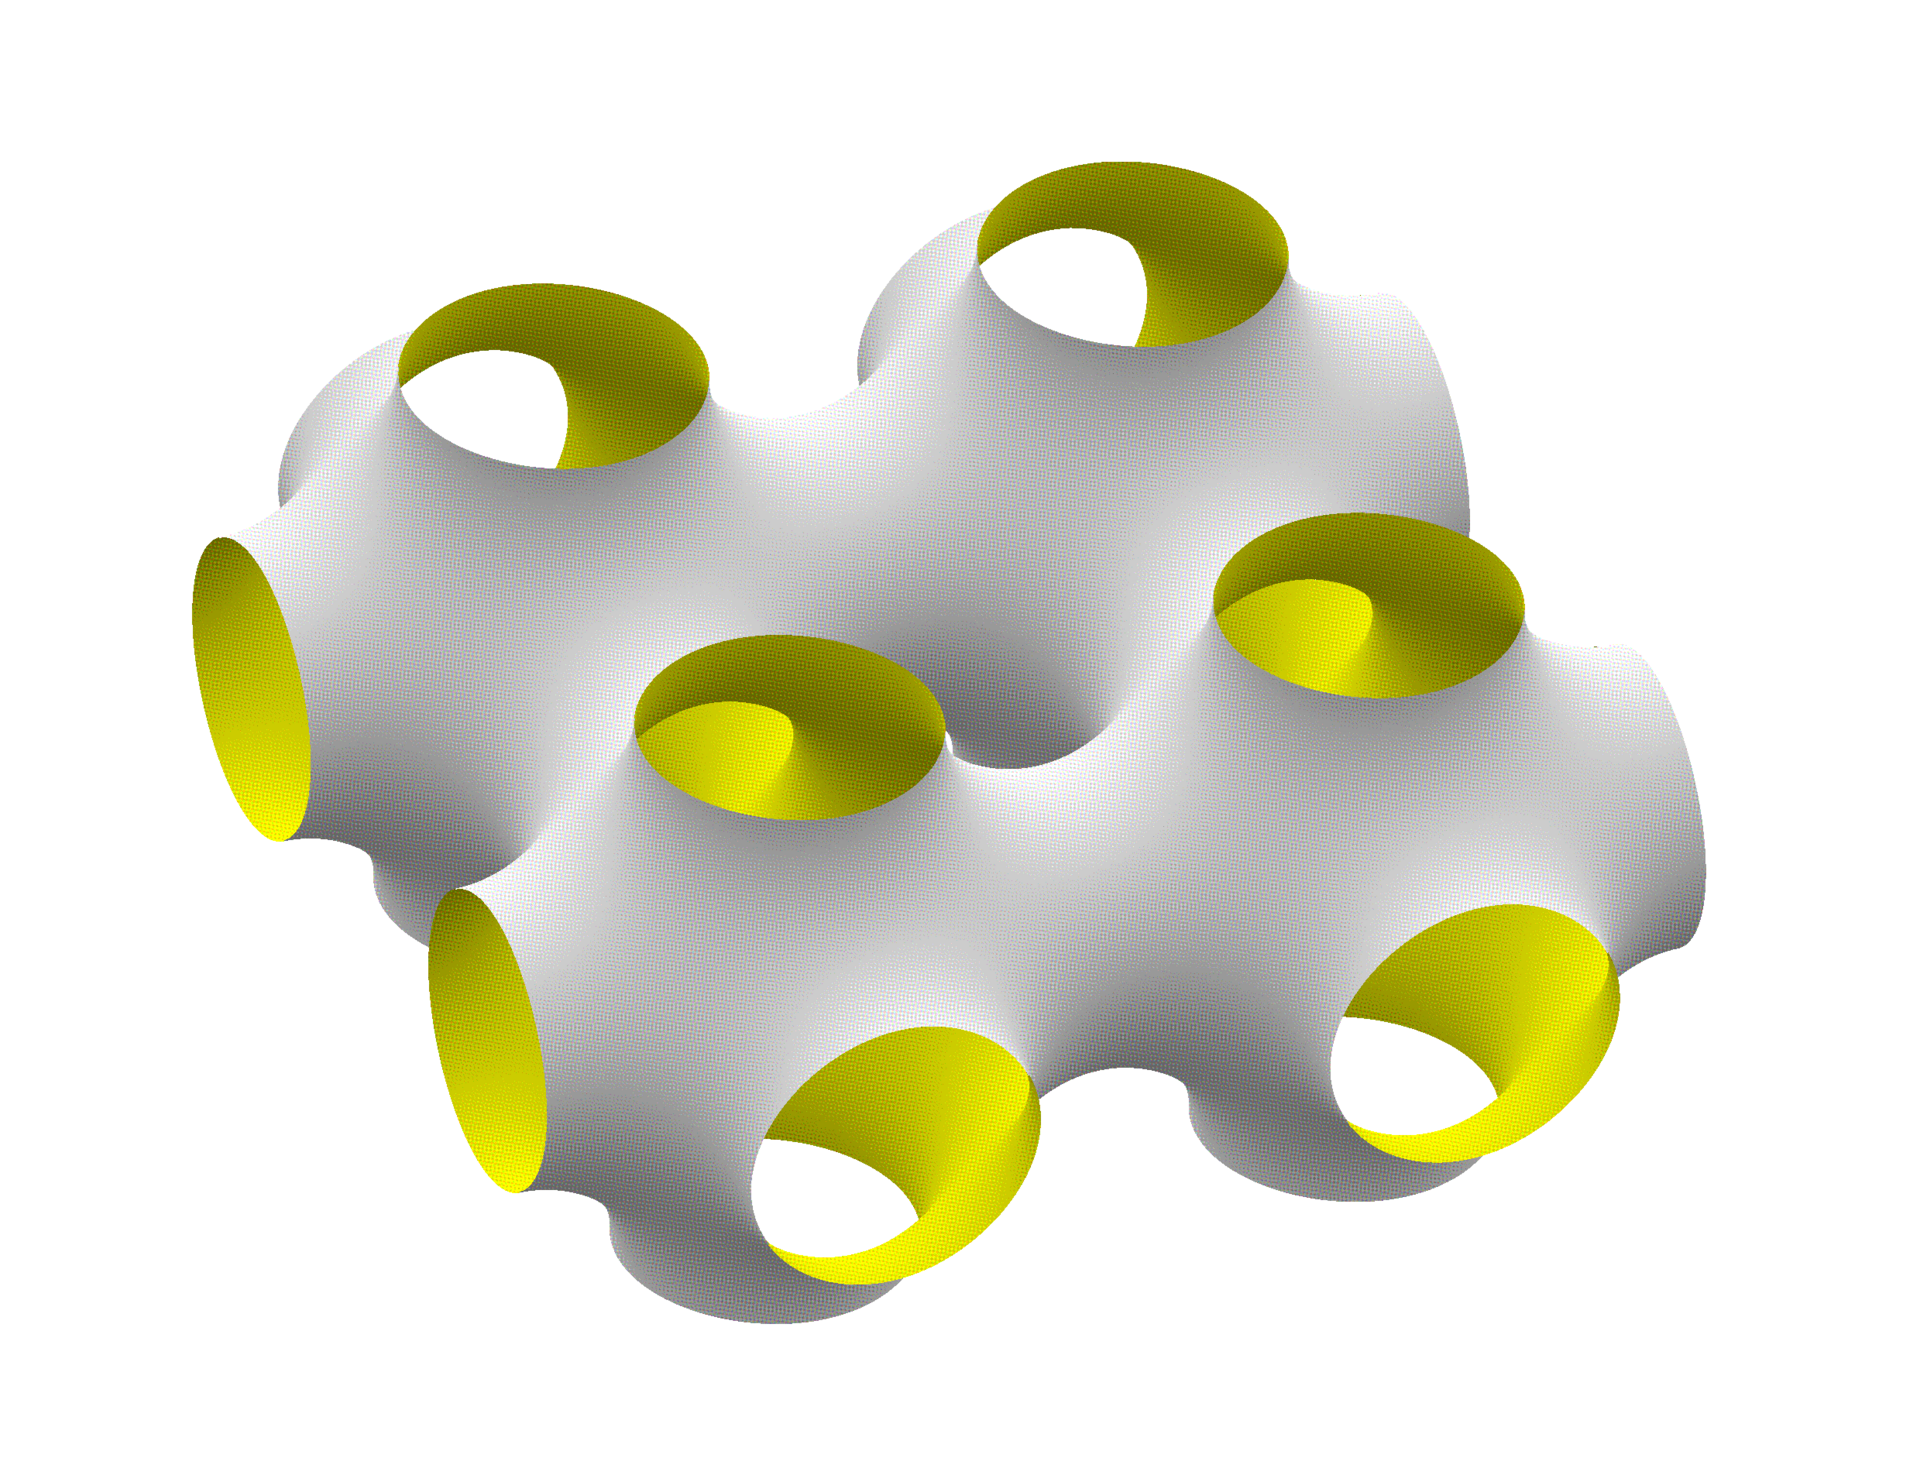
\includegraphics[width=0.5\textwidth]{fig1}
\end{figure}
You can think of this as put inside 3-torus \(\mathbb{T}^3\overset{\operatorname{def}}{=}\mathbb{R}^3/\mathbb{Z}^3\).
\end{example}

\begin{example}\leavevmode
Enneper surface.
\iffalse\begin{figure}[H]
	\centering
	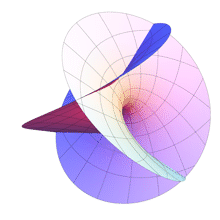
\includegraphics[width=.5\textwidth]{fig2.png}
\end{figure}\fi
\end{example}

*We saw several other examples* In conclusion, minimal surfaces exist and you can see some of them.

\subsection{Basic objects}

Consider
\[M^{(m)}\overset{f}{\hookrightarrow }N^{(n)}=\mathbb{R}^n,\qquad x_1,\ldots,x_n\]
It has a differential
\[T_pM \longrightarrow T_{f(p)}N=\mathbb{R}^n\]
which is a linear map. Now take local coordinates \(D \subset M\), \((u_1,\ldots,u_n)\). Then \(f \) is locally fiven by a functions of \(m\) variables
\begin{align*}
	x_1(u_1,\ldots,u_m)\\
	\vdots \\
	x_n(u_1,\ldots,u_m)
\end{align*}
while \(df_p\) is represented by a \(m\times n\) matrix
\[\left(\frac{\partial x_i}{\partial u_J}\right) ,\qquad  i=1,\ldots,n, j=1,\ldots,m\]
If \(N^{(n)}\cong M^{(m)}\times \mathbb{R}^{n-m}\) and \(f= \operatorname{id}_M \times \varphi\) (so \(M = \Gamma_\varphi\) a graph of \(\varphi\). Then we get a matrix
\[\begin{pmatrix} \operatorname{Id} & * \end{pmatrix} \]
Now look again at \(M \overset{f}{\hookrightarrow }N\). We can pull back the metric of \(N\), which is a symmetric tensor, getting a metric on \(M\). ({\color{6}dani: because \(f\) is immersion=differential is injective).}

So let's try to see how this metric looks like. The pullback metric should of course be something of the kind
\[\sum g_{j j'} du_j du_{j'}\]
now since \(g= \sum (dx_i)^2\) is euclidean metric we get
\[\sum \left(\sum \frac{\partial x^i}{\partial u_j}du_j\right)^2 \]
so that
\[g_{j_1j_2}= \sum \frac{\partial x^i}{\partial u_{j_1}}\frac{\partial x^i}{\partial u_{j_2}}\]
So if this matrix is \(G\) and \(J\) is the jacobian of \(f\) we just get
\[G=J^{\mathbf{T}}J\]

\begin{remark}\leavevmode
We could also just define a metric on \(M\) by putting those coefficient functions and create s symmetric 2-tensor.
\end{remark}
Now consider
\[\bar{g} :=\det(g_{ij})\]
if \(\bar{g}\neq 0 \) then matrix  \((g_{ij})\) is invertible, so it has inverse \((g^{ij})\).

\begin{thing8}{Definition/Proposition}\leavevmode
\(f\) is \textit{\textbf{regular}} in a point \(p\) if any of these equivalent conditions hold:
\begin{enumerate}
\item \(\bar{g}\neq 0\).
\item \(\bar{g}>0\).
\item Vectors \(\left(df_p\right) \left(\frac{\partial }{\partial u_i}\right) \) are linearly independent.
\end{enumerate}
\end{thing8}

\begin{proof}\leavevmode
\end{proof}

\begin{defn}[Cotangent and tangent space]\leavevmode
For a local system of coordinates we can define
\[\Omega_{\mathbb{R}^n}:=\left<dx^{(1)},\ldots,dx^{(n)}\right>\]
as the space generated by the differentials of the coordinate functions. Then we define
\[T_{\mathbb{R}^n}:=\left<\frac{\partial }{\partial x^{(1)}},\ldots,\frac{\partial }{\partial x^{(n)}}\right>\]
as generated by the dual basis of the cotangent basis.
\end{defn}

\subsection{Volume of a submanifold of \(\mathbb{R}^n\)}

Consider \(U,V\) vector spaces and
\[\begin{tikzcd}
	U \arrow[r,"T"]& U \arrow[ r,"\sharp_g"]\arrow[r,"\cong",swap]&  U^{\vee}\arrow[r,"T^*"]&  U^{\vee}
\end{tikzcd}\]
where \(g\) is a metric on \(V\). Then the composition of all this is just the same as the pullback metric on \(U\)! 
\[T^*  \circ \sharp_g \circ T=\sharp_{T^*g}:U \to U^{\vee}\]
Now apply \(\Lambda^{m}\) to get another commutative diagram
\[\begin{tikzcd}
	\Lambda^{m}U \arrow[ r,"\Lambda^{m}T"]\arrow[rrr,bend right,"\bar{g}"]\arrow[d,equals]&\Lambda^{m}V\arrow[r,"\Lambda^{m}\sharp g"]&\Lambda^{m}V^{\vee}\arrow[ r,"\Lambda^{m}T^{\vee}"]&  \Lambda^{m}U^{\vee}\arrow[d,equals]\\
	\mathbb{R}& & & \mathbb{R}
\end{tikzcd}\]
and then the composition here gives us
\[\bar{g}=\sum_{1\leq  j_1\leq \ldots \leq j_m \leq n}\left(\det\left(\frac{\partial x^{j_k}}{\partial u_i}\right) \right) ^2\]

Let \(v_1,\ldots,v_n\) be a basis of \(U\) and \(e_1,\ldots,e_n\) another basis. Let \(V\) be a matrix that takes one basis to another. Then
\[G=V^{\mathbf{T}}V\]
\[\implies \det G= \det(V)^2\implies \bar{g}(p)=\operatorname{Vol}_M\Big((df)_p\left(\frac{\partial }{\partial u_1}\right),\ldots,(df)_p\left(\frac{\partial }{\partial u_n}\right) \Big)^2 \]

\begin{defn}[Volume of \(M \overset{f}{\hookrightarrow }\mathbb{R}^n\)]\leavevmode
 \[\operatorname{Vol}M=\int_M\sqrt{\det g}du_1\ldots du_m \]
\end{defn}

Which takes us to the problem of volume minimzation.

Then followed some computation of the minors of
\[\begin{pmatrix} 1&0&z_x\\0&1&z_y \end{pmatrix}\ldots \]

\begin{thing6}{Extra, we discussed this at some time}\leavevmode
That \textit{\textbf{hypersurface}} is a thing locally defined by \textit{one} function.
\end{thing6}

\section{Class 3}

\subsection{Isothermic coordinates}

A \textit{\textbf{Weyl transformation}} is a map of metrics
\[g \mapsto  e^kg\]
where we use exponent just to mean an invertible positive number. \(k\) is a real function.

\begin{upshot}\leavevmode
That a metric on a surface induces a complex structure given by anticlockwise 90-degree rotation. And the interesting part is that two conformal metrics induce the same conformal structure, and the map that relates these metric is the Weyl transform.
\end{upshot}

\begin{thing8}{Example: euclidean coordinates}\leavevmode
Euclidean metric is \((du)^2+(dv)^2\). Letting \(dz:=du+idv\) and \(d\bar{z}:=du-i dv\) we get
\[(du)^2+(dv)^2=(dz)\cdot(d\bar{z})\]
Now take other coordinates \(w\), \(w=F(z)\).  You'll get
\[dw\cdot d \bar{w}=\underbrace{|F^i(z)|^2}_{e^k}dz\cdot d\bar{z}=e^k((du)^2+(dv)^2)\]
And the matrix is
\[\begin{pmatrix}e^k&0\\ 0&e^k\end{pmatrix}\]

\textbf{Conclusion:} conformal class of metric is the same as complex structure.
\end{thing8}

\begin{defn}\leavevmode
\textit{\textbf{Isothermic coordinates}} are local coordinates \((u,v)\) such that \(g_{11}=g_{22}\) and \(g_{12}=0\). So,  \textbf{scalar} multiple of euclidean metric.
\end{defn}


\begin{claim}\leavevmode
Any Riemannian surface \((\Sigma,g)\) has local isothermic coordinates. (In fact, for every power series we get another isothermic coordinates. There is a group action of the \textit{\textbf{local biholomorphisms}}. In higher dimension this is only finite dimensional, generated by inversions (this is a group, like inversion about circle in \(\mathbb{C}\) and isometries (i.e. \(\operatorname{Isom}(\mathbb{R}^n) \supset\mathsf{O}(n),\mathbb{R}^n\)). So conclusion: in dimension 2 it has to do with complex analysis and in higher dimension it's just different.)
\end{claim}

\begin{thing7}{We have learnt}\leavevmode
that there are some thing of complex analysis like maximum principle and probably also Schwarz principle that generalize to higher dimension, but not everything.
\end{thing7}

\begin{remark}\leavevmode
Recall that conformal maps are either holomorphic or antiholomorphic.
\end{remark}

\subsection{Grassmanian}

Recall what is grassmanian \(\operatorname{Gr}(m,n)\) with \(m<n\), the variety of \(m\)-dimensional vector subspaces of an \(n\)-dimensional vector space \(V\), and Plucker embedding \(\operatorname{Gr}(m,n)\hookrightarrow \mathbb{P}\Lambda^{m}V\).


\begin{defn}\leavevmode
\(V\) has \textit{\textbf{vectors}}. \(V^\vee\) has \textit{\textbf{covectors}}.  \(\Lambda^{2}V\) has \textit{\textbf{bivectors}}.  \(\Lambda^{3}V\) \textit{\textbf{trivectors}}.  \textit{\textbf{Polyvectors}}. For bundles:  \(\Lambda^{2}T_M\) \textit{\textbf{bivector fields}}.  \(\Lambda^{m}T_M\) \textit{\textbf{polyvector (or multivector) fields}}, they are dual to  \(\Omega^{m}=\Lambda^{m}\Omega\), differential \(m\)-forms.
\end{defn}
For a subspace \(U \subset V\) we get corresponding \(\underbrace{\Lambda^{m}U }_{\substack{\text{1-dim casr}  \\ \cong\mathbb{R}}}\xrightarrow{\Lambda^{m}j}\Lambda^{m}V\)
and corresponidingly
\[\underbrace{\mathbb{P}\Lambda^{m}U}_{\substack{\text{1 dim}  \\ =pt}}\xrightarrow{\mathbb{P}(\Lambda^{m}j)}\mathbb{P}\Lambda^{m}U\]

Next. If \(V=\mathbb{R}^n\) is equipped with a metric \(g\) you have for two orthonormal bases
\[e_1 \wedge \ldots \wedge e_m=\det C f_1\wedge \ldots \wedge f_m\]
For a map \(f_i=C_i^j e_j\). If they are orthonormal you get \(\det C=\pm 1\) and of you orient it all you get \(\det C=1\).

Correspondingly define the space of \textit{oriented} vector subspaces of euclidean space by \(\operatorname{Gr}^+(m,\mathbb{R}^n)\).
For a basis \(U=\left<u_1,\ldots,u_m\right>\), we get a basis \(\Lambda^{m}U=\left<u_1\wedge u_2\wedge\ldots \wedge u_m\right>\).


\begin{example}\leavevmode
\begin{itemize}
\item \(\operatorname{Gr}(1,2)=\) circle.
\item \(\operatorname{Gr}^+(1,2)\) space of rays.
\item \(\operatorname{Gr}^+(1,\mathbb{R}^n)=S^{n-1}\).
\item \(\operatorname{Gr}(1,\mathbb{R}^n)=\mathbb{R}P^{n-1}\).
\end{itemize}
\end{example}

Now do
\[\begin{tikzcd}0\arrow[r]&U^{(m)}\arrow[r]&V^{(n)}\arrow[r]&Q^{(n-m)}\arrow[r]&0\end{tikzcd}\]
dualize
\[\begin{tikzcd}0\arrow[r]&Q^\vee\arrow[r]&V^\vee\arrow[r]&U^\vee\arrow[r]&0\end{tikzcd}\]
So you automatically get isomorfphism
\[\operatorname{Gr}(m,V)=\operatorname{Gr}(V,n-m)=\operatorname{Gr}(n-m,V^\vee)=\operatorname{Gr}(V^\vee,m)\]
And now pick some orientation on \(V\), you shall get 
\begin{exercise}\leavevmode
\(\Lambda^{n}V \cong \Lambda^{m}U \otimes \Lambda^{n-m}Q\)
\end{exercise}

\begin{example}\leavevmode
\(\operatorname{Gr}^+(2,3)=S^2=\) conic \(\subset\mathbb{C}P^{2}\), more exactly \(\{x^2+y^2+z^2=0\}\).
\end{example}

\begin{exercise}\leavevmode
\(\operatorname{Gr}^+(2,\mathbb{R}^n)\cong Q^{n-2}\subset \mathbb{C}P^{n-1}\) of the form \(\left\{\sum_{i=1}^n z_i^2=0\right\}\)
\end{exercise}

\subsection{ Now}
Consider 
\[M^{(m)}\xrightarrow{f}N^{(2)}\]
and do
\[\mathbb{R}^m \cong T_p^m M \xrightarrow{d_pf}T_{f(p)}N \cong \mathbb{R}^n\]
so for every regular (=rank is \(m\)=the map is an embedding=the thing is a subvariety) \(p\) you get a point in grassmanian
\[\operatorname{Gr}(m,T_{f(p)}N)\]
Consider \(f^*T_N\) which is a vector bundle over \(M\), then we can consider
\[(df):T^{(m)}_M \overset{\text{by regularity,} }{\hookrightarrow } f^*T^{(n)}_N \to \underbrace{f^*(T_N / df(T_M))^{n-m}}_{\text{\textit{\textbf{normal bundle}}} }\]
and then consider the \textit{\textbf{Grassmanization}} of \(f^*T_N\), which is a bundle
\[\begin{tikzcd}
\operatorname{Gr}(m,f^*T_N)\arrow[d]\\
M
\end{tikzcd}\]
Now consider sections of this thing.

\begin{thing7}{Important observation}\leavevmode
 Given a trivialization of \(f^*T_N\), a section of the thing becomes just a map
 \[M \to \operatorname{Gr}(m,n)\]
 (Because a section of a trivial bundle is just a map to the fiber.) 
\end{thing7}

Now fix \(N:= \mathbb{R}^n\) and put a connection, the Levi-Civita connection. Actually now better take the oriented Grassmanian for the whole bussiness. And we have the map
\[M \to \operatorname{Gr}^+(m,n)\]
which is a map that to every point associates its tangent space. And it is called the \textit{\textbf{Gauss map}}.

Recall that
\begin{claim}\leavevmode
A surface is minimal \(\iff\) Gauss map is conformal (anti-holomorphic).
\end{claim}

Put a surface in \(\mathbb{R}^3\). Basis for tangent space is
\[(x_u,y_u,z_u), (x_v,y_v,z_v)\]
So basis for projectivization is
\[(y_uz_u-y_vz_u, x_uz_v-x_vz_u,x_uy_v,x_vy_u)\]
and in general, when you get
\begin{align*}
\Sigma&\to \mathbb{R}^n\\
\frac{\partial }{\partial u}x, \frac{\partial }{\partial v}X &\rightsquigarrow \frac{\partial x}{\partial u}\wedge \frac{\partial x}{\partial v}
\end{align*}
\begin{thing8}{Lesson}\leavevmode
Plücker coordinates of oriented Grassmanian are the same as coordinates of normal bundle!
\end{thing8}
But also notice that you can write
\[\{x^i,x^j\}_{du \wedge dv}\]
And the point of all this is that 

\begin{claim}\leavevmode
Minimal surfaces are equivalently defined as the ciritical points of the \textit{\textbf{Schild action}} 
\[\int \left(\sum_{i<j}\{x_i,x_j\}^2\right)\omega\]

\end{claim}
Now put a curve \(I \subset \Sigma \to \mathbb{R}^n\)… [what was the curve for…?]

\begin{thing7}{Hint}\leavevmode
From 1 to 2 you ``vary" the volume and look for critical points.
\end{thing7}

\begin{thing6}{Important exercise}\leavevmode
If \(x=u,y=v\) and \(z=\varphi(u,v)\), you get two derivatives
\[\partial_u \to (1,0,\varphi_u)\qquad \partial_v \to (0,1,\varphi_v)\]
Notice that
\[df[\partial_u]=\partial_x+\varphi_u\cdot \partial_z\]
And now
\[\partial_u \wedge \partial_v = \partial_u \wedge \partial_y- \varphi_v\partial_x \wedge\partial_z-\varphi_v \partial_y \wedge \partial_z\]
Then you have proportionality
\[N \sim (-\varphi_u,-\varphi_v,1):=\tilde{N}\]
So
\[\|\tilde{N}\|^2=\varphi_u^2+\varphi_v^2+1=g\]
\[N=\frac{\tilde{N}}{\sqrt{g} }\]
So \textit{\textbf{Gauss map for non-parametric surface}} is 
\[G:(u,v) \longrightarrow\left(\frac{-\varphi_u}{\sqrt{1+\varphi^2_u+\varphi^2_v} },\frac{-\varphi_v}{\sqrt{1-\varphi^2_u+\varphi^2_v} },\frac{1}{\sqrt{1-\varphi_u^2+\varphi_v^2} }\right) \]
(and you can just write \(\sqrt{1+\varphi_u^2+\varphi_v^2} =\sqrt{g} \) but Ok). Similarly…
\end{thing6}

And differentiate!
\[dG:T_pM \to T_{G(p)}\operatorname{Gr}(m,n)=\operatorname{Hom}(T_pM,\text{Normal bandle}N )\]
So you see
\[dG \in \operatorname{Hom}(T_pM,\operatorname{Hom}(T_pM, N))\]
So it's a map
\(T_pM \times T_pM \to N\) 
But \(N\) is trivialized! So you can think of  \textit{numbers}. So it's a form.

\begin{claim}\leavevmode
That map is symmetric.
\end{claim}
So you can define it to be the \textit{\textbf{second fundamental form}}.


\begin{thing8}{Notations}\leavevmode
\begin{itemize}
\item I fundamental form \(\rightsquigarrow \) \(g_{ij}\).
\item  II fundamental form \(\rightsquigarrow \) \(B_{ij}\) for a vector in the normal bundle, and \(b_{ij}\) when you are in \(\mathbb{R}^3\) and you have trivialized it to get numbers
\end{itemize}
\end{thing8}

\begin{claim}\leavevmode
\[B_{ij}=\left(\frac{\partial^2 \vec{x}}{\partial u_i\partial u_j}\right)^N \]
where exponent \(N\) means projection to the normal bundle which can mean algebraic projection when you think of a quotient bundle or orthogonal projection when you think geometric.
\end{claim}

\begin{thing6}{Reminder of the end of last lecture}[Variation of the tangent direction]\leavevmode
	\begin{align*}V'(t=0)[\underbrace{\delta \varphi}_{:=w}]= \int_{\Sigma}\frac{z_x\cdot w_x+z_y\cdot w_y}{\sqrt{g} }dudv\\
		&=\int \left<\delta \varphi,\text{something} \right>\frac{\sqrt{g} dudv}{\text{volume form} }
	\end{align*}
where \(\delta \varphi\) is a section of \(f^* T_{\mathbb{R}^n}=df(T_M) \oplus^\perp N\). And \textbf{something} is a unique thing that exists making the equality hold. This is a possible definition of \textit{\textbf{mean curvature vector}} \(\vec{H} \in N\).

And you can also write
\[\int dv \wedge \left(\frac{z_u}{\sqrt{g} \cdot w_u du}\right) = \int dv \wedge \left(\frac{z_u}{\sqrt{g} }dw\right) \]
where \(dw=w_u du+\ldots+dv\). And now we want to integrate by parts so if you recall
\[=-\int w \cdot \partia\left(\frac{z_u}{v_g}dv\right) \]
So the integral above becomes
\begin{align*}
\int_{\Sigma}\frac{z_x\cdot w_x+z_y\cdot w_y}{\sqrt{g} }dudv&=-\int \left(\partial_u \left(\frac{z_u}{\sqrt{g} }\right)+\left(\partial_v \frac{z_v}{\sqrt{g} } \right) \cdot w du dv
\end{align*}
so if that is zero for all \(w\).
\end{thing6}

Right so that is the \textit{\textbf{first variation of volume}}? It's
\[V'|_{t=0}=-\int_\Sigma(\sqrt{g} du) \left<H,W\right>\]
And it has all to do with the expression \(\Sigma g^{ij}B_{ij}\).




\clearpage\bibliography{bib.bib}
\end{document}
